

\subsubsection{Methodology}

Logistic regression is a regression model that estimates the \textit{log-odds} of an event as a linear combination of features:

\begin{align*}
    \ln \frac{\hat p}{1 - \hat p} = \hat\beta_0 + \hat\beta_1 X_1 + \cdots + \hat\beta_k X_k
\end{align*}

where \( \hat p \) is the estimator of \( \mathbb P[Y = 1] \), \( \hat\beta_0, \hat\beta_1, \cdots, \hat\beta_k \) are estimates of the linear coefficients. Unlike the usual linear regression, logistic regression has less assumption on its variable. For example, normality of independence variables is not required, hence it is not expected that logistic regression would better-fit on standardised data than the original one.

\begin{figure}[h]
    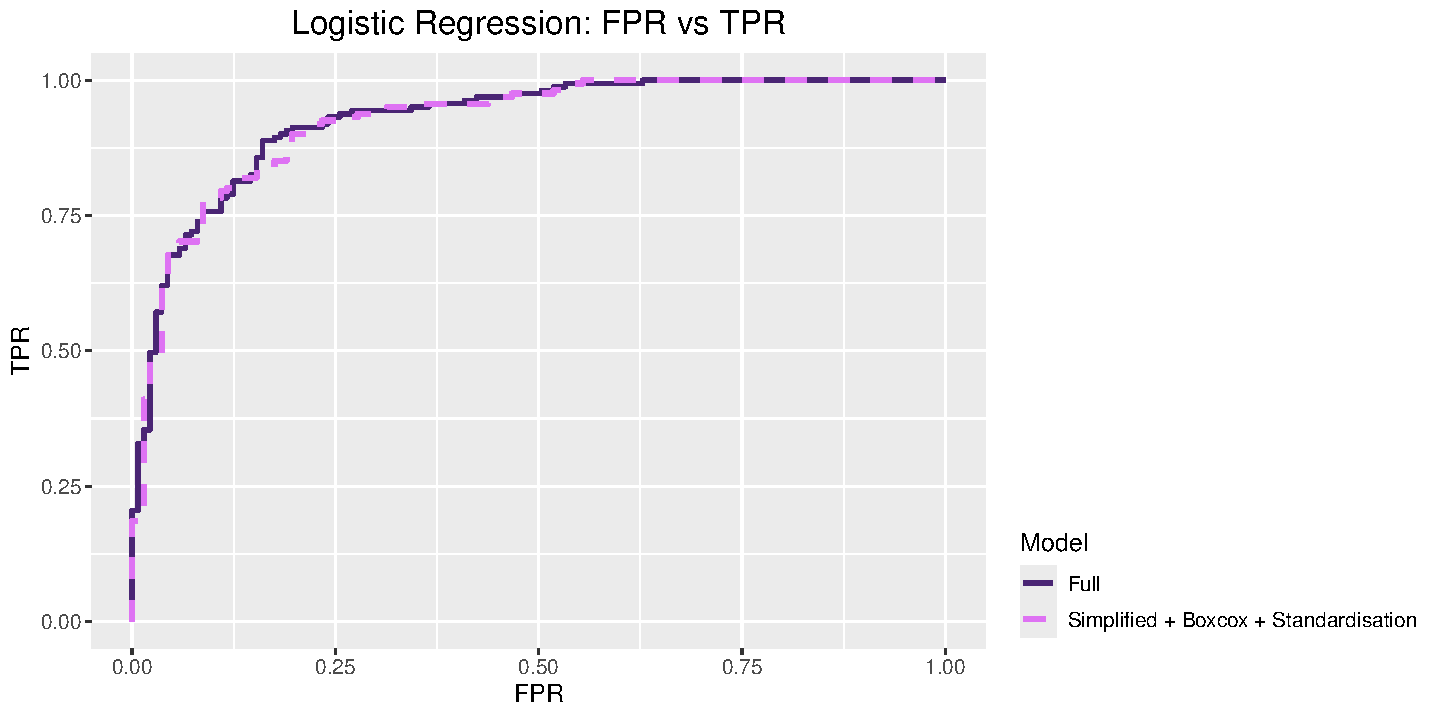
\includegraphics[width=\linewidth]{33.LogisticRegression.pdf}
    \caption{\centering ROC curve for logistic models}
\end{figure}

\subsubsection{Experiments \& Results}
Indeed, two logistic models are tested, a full model on all \( 12 \) features, and a simplified model on a Box-Cox, standardised version of only \( 9 \) significant features. They yields relatively similar results: investigation on the ROC curves produced by the two models shows that they pretty much overlap, except when \( \textrm{FPR} \approx 0.125 \) when the curve of the simplified model concaves down.

% \begin{table}[h]
%     \centering
%     \begin{tabular}{ccc}
%         \toprule
%         Logistic Regression
%             & \textbf{Full}
%             & \textbf{Box-Cox, Simplified\footnotemark{}}
%         \\
%         \midrule
%         \textbf{AUC}
%             & \( 0.9268 \)    
%             & \( 0.9235 \)
%         \\
%         \bottomrule
%     \end{tabular}
    
%     \raggedright
%     \( ^2 \) {\small \texttt{fbs}, \texttt{bp} and \texttt{chol} are excluded from the model}
    
%     \centering
%     \vspace{4pt}
%     \caption{}
% \end{table}

It can also be seen from the model coefficients that features contributing the most to the prediction of disease include \texttt{chest.pain}, \texttt{sex}, \texttt{blood.disorder} and \texttt{vessels}. There is a similarity between logistic models and decision trees, in the sense that these set of features stand as strong predictors for disease.

\begin{table}[h]
    \centering
    \begin{tabular}{lrr}
        \toprule
        \textbf{Feature} & \textbf{Estimate\footnotemark{}} & \textbf{p-value}\\
        \midrule
        \bf chest.pain3 & \bf 1.88 & \bf 0.0031\\
        \midrule
        \bf chest.pain2 & \bf 1.86 & \( \bf <  0.0001 \) \\
        \midrule
        \bf sex1 & \bf -1.31 & \bf 0.0085\\
        \midrule
        blood.disorder3 & -1.28 & 0.0954\\
        \midrule
        \bf chest.pain1 & \bf 1.11 & \bf 0.0437\\
        \midrule
        \bf vessels & \bf -0.80 & \( \bf < 0.0001 \)\\
        \midrule
        angina1 & -0.76 & 0.0716\\
        \midrule
        \bf st.depression & \bf -0.69 & \bf 0.0040\\
        \midrule
        rest.ecg1 & 0.65 & 0.0785\\
        \midrule
        \bf heart.rate & \bf 0.53 & \bf 0.0242\\
        \midrule
        (Intercept) & 0.44 & 0.6332\\
        \midrule
        rest.ecg2 & -0.30 & 0.8992\\
        \midrule
        \color{red}{chol} & 0.30 & 0.1504\\
        \midrule
        \color{red}{bp} & 0.29 & 0.1213\\
        \midrule
        blood.disorder2 & 0.21 & 0.7880\\
        \midrule
        \color{red}{fbs1} & 0.19 & 0.7367\\
        \midrule
        age & 0.01 & 0.9661\\
        \bottomrule
    \end{tabular}

    \raggedright
    \( ^\# \) {\small \textbf{bold values} indicate significant features (\( \alpha = 0.05 \))}
    
    \( ^3 \) {\small sorted by magnitude of coefficients}

    \centering
    \vspace{4pt}
    \caption{Description of the logistic model}
\end{table}

